\documentclass[a4paper, 12pt, english]{article}

\usepackage[utf8]{inputenc}
\usepackage{amsmath, amssymb}
\usepackage{graphicx}
\usepackage{subfig}
\usepackage{indentfirst}
\usepackage{verbatim}
\usepackage{textcomp}
\usepackage{gensymb}
\usepackage{relsize}
\usepackage{float}
\usepackage[backend=biber]{biblatex}
% \usepackage[colorinlistoftodos]{todonotes}

\addbibresource{references.bib}

\usepackage{lipsum}% http://ctan.org/pkg/lipsum
\usepackage{xcolor}% http://ctan.org/pkg/xcolor
\usepackage{xparse}% http://ctan.org/pkg/xparse
\NewDocumentCommand{\myrule}{O{1pt} O{2pt} O{black}}{%
    \par\nobreak % don't break a page here
    \kern\the\prevdepth % don't take into account the depth of the preceding line
    \kern#2 % space before the rule
        {\color{#3}\hrule height #1 width\hsize} % the rule
    \kern#2 % space after the rule
    \nointerlineskip % no additional space after the rule
}


\usepackage[section]{placeins}

\usepackage{booktabs}
\usepackage{colortbl}
\newcommand{\myrowcolour}{\rowcolor[gray]{0.925}}

\usepackage{etoolbox}
% \usepackage{obeyspaces}{url}

\usepackage{hyperref}
\hypersetup{
    colorlinks,
    citecolor=black,
    filecolor=black,
    linkcolor=black,
    urlcolor=black
}

\usepackage{geometry}
\geometry{
    paper=a4paper, % Change to letterpaper for US letter
    inner=3cm, % Inner margin
    outer=3cm, % Outer margin
    bindingoffset=.5cm, % Binding offset
    top=2cm, % Top margin
    bottom=2cm, % Bottom margin
% showframe, % Uncomment to show how the type block is set on the page
}
%*******************************************************************************%
%************************************START**************************************%
%*******************************************************************************%
\begin{document}

%************************************TITLE PAGE**************************************%
    \begin{titlepage}
        \begin{center}
            \textbf{\LARGE Politecnico di Torino}\\[0.5cm]
            \textbf{\large DEPARTMENT OF AUTOMATICS AND COMPUTER SCIENCE}\\[0.2cm]
            \vspace{20pt}
            
\includegraphics[scale=0.5]{img/title/logo-polito}\\[0.5cm]

            \par
            \vspace{20pt}
            \textbf{\Large 01URTOV MACHINE LEARNING AND PATTERN RECOGNITION}\\
            \vspace{30pt}
            \myrule[1pt][7pt]
            \textbf{\LARGE  PROJECT REPORT}\\
            \vspace{15pt}
            \textbf{\large Data Analysis and Pattern Recognition}\\
            \myrule[1pt][7pt]
            \vspace{25pt}
            \makebox[3cm][c]{\textbf{\large Student Name}}\hspace{25pt}\makebox[3cm][c]{\textbf{\large Student ID}}\\
            \makebox[3cm][c]{Taormina Nicolò}\hspace{20pt}\makebox[3cm][c]{331853}\\

            \vspace{55pt}
            \textbf {\large Lecturer in charge:}\\[0.2cm]
            \Large {Cumani Sandro}\\[0.1cm]
        \end{center}

        \par
        \vfill
        \begin{center}
            \textbf{Compilation Date: \today}\\
        \end{center}

    \end{titlepage}
%************************************TABLE OF CONTENTS**************************************%

%Summary
    \newpage
    \tableofcontents
% \thispagestyle{empty}
%End Summary

%********************************%
%***********Premise**************%
%********************************%
    \newpage
    \section*{Premise}
    All the code that will follow is publicly available and free to use at my personal GitHub \cite{nickrepository}


    \addcontentsline{toc}{section}{Premise}
%********************************%
%**********INTRODUCTION**********%
%********************************%
    \section*{Introduction}
    The following section will introduce and answer all the relative question regarding the project in examination, but before it is important to clarify that to avoid cluttering the plot with repetitive information, it may happen that the legend would not be present in all the individual plot, still the necessary information will always be present to correctly read the figures presented in the following pages.
    As an example, using the following figure that is used to answer the first question:
    \begin{figure}[H]
        \centering
        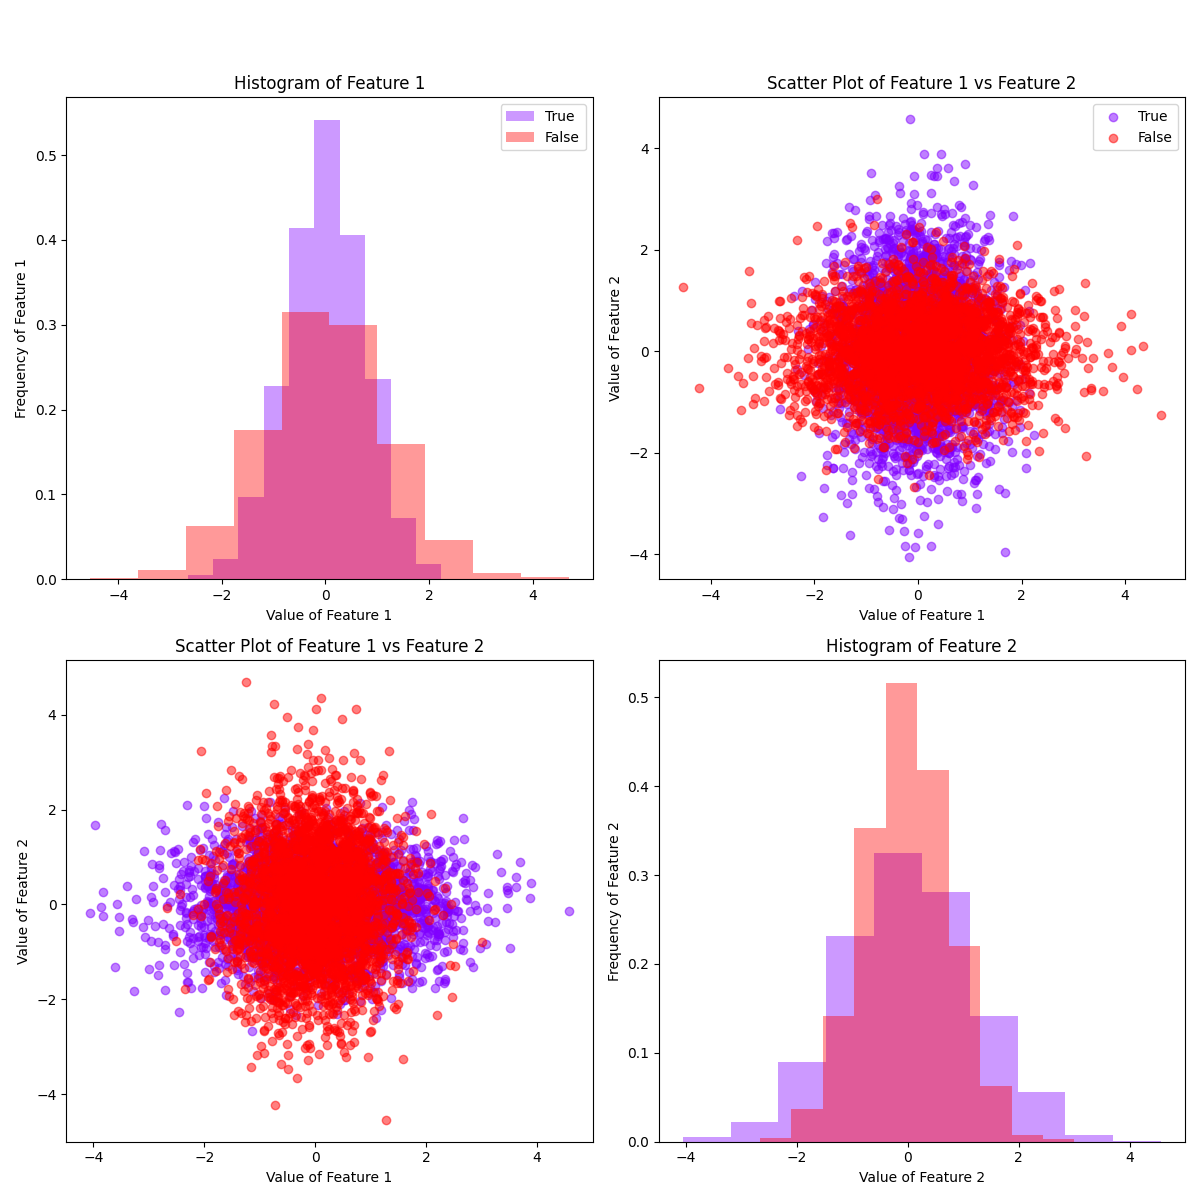
\includegraphics[width=0.7\linewidth]{img/projects/project1/1-2.png}
        \caption{First and Second features}
        \label{fig:project1:1-2}
    \end{figure}
    here the legend show the color only for the first histogram and the first scatter plot, but the same colors apply for the remaining, such that the second scatter plot has the \textit{blueish} color for the \textbf{\textit{True}} class and the \textit{reddish} color for the \textbf{\textit{False}} one. The same apply for the second histogram, as that \textit{blueish} is the \textbf{\textit{True}} class and \textit{reddish} is the \textbf{\textit{False}} class. Colors may change from figure to figure, but the consistency will remains inside the same figure.

    \addcontentsline{toc}{section}{Introduction}
%********************************%
%***********Project 1************%
%********************************%
    \newpage


    \section{Project 1}

    \subsection{Questions}
    \begin{enumerate}
        \item Analyze the first two features. What do you observe? Do the class overlap? If so, where? Do the class show similar mean for the first two features? Are the variances similar for the two classes? How many modes are evident from the histograms (i.e., how many “peaks” can be observed)? \hyperref[project1:1]{[\textbf{Answer}]}.
        \item Analyze the third and fourth features. What do you observe? Do the class overlap? If so, where? Do the class show similar mean for the first two features? Are the variances similar for the two classes? How many modes are evident from the histograms? \hyperref[project1:2]{[\textbf{Answer}]}.
        \item Analyze the last two features. What do you observe? Do the class overlap? If so, where? How many modes are evident from the histograms? How many clusters can you notice from the scatter plots for each class? \hyperref[project1:3]{[\textbf{Answer}]}.
    \end{enumerate}

    \subsection{Answers}

    \subsubsection{First and Second Features}
    \label{project1:1}
    The first approach to analyze the two features could be a visual one, using the \hyperref[fig:project1_1-2]{\textit{figure}} produced by the Matplotlib library \cite{Hunter:2007} available for the python language.
    \begin{figure}[H]
        \centering
        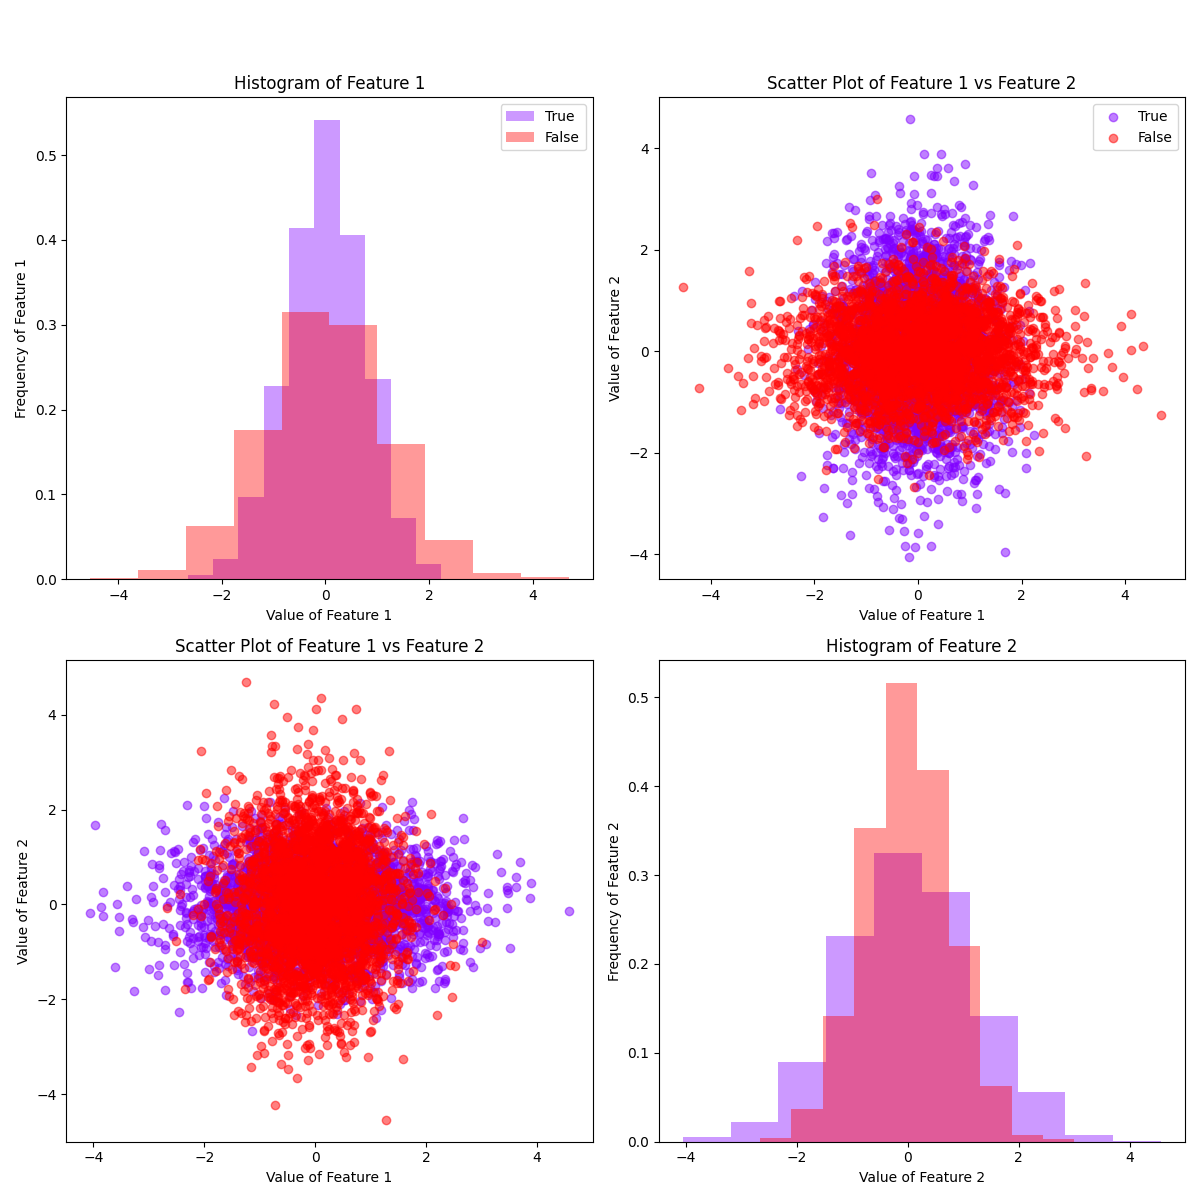
\includegraphics[width=0.7\linewidth]{img/projects/project1/1-2.png}
        \caption{First and Second features}
        \label{fig:project1_1-2}
    \end{figure}

    Visually it is possible to notice four modes: two for each feature and a single mode for each class, all of them near the zero value, although the mode for the “False” class for the first features is much less prominent. From this first analysis and some visual deducting, it is possible to determine a very similar value for both the mean and variance of the first two features, but it is not possible to determine precisely what it is (the mean is obviously near the zero value).
    Calculating the actual value confirm the visual hypothesis of centered means and similar variance as the mathematical value are:
    \begin{table}[htbp]
        \centering
        \begin{tabular}{|c|c|c|}
            \hline
            & \textbf{Feature 1}   & \textbf{Feature 2}   \\
            \hline
            \textbf{Mean}     & 0.001707107265713465 & 0.005039029435563128 \\
            \hline
            \textbf{Variance} & 1.001343035018908    & 0.9983526991183364   \\
            \hline
        \end{tabular}
    \end{table}

    Thus, both visually and analytically confirming a great overlap of the two classes and the features. The last one can be noted from their similarity in the mean and variance.
    Another intuition is the different variance the two classes show for each feature:
    \begin{enumerate}
        \item Feature 1: \textbf{True} class has an high peak with little variance, unlike the \textbf{False} class that has a lower peak with higher variance.
        \item Feature 2: the opposite of the first feature as the \textbf{True} class present with a lower peak and higher variance then the \textbf{False} class

    \end{enumerate}

    \subsubsection{Third and Fourth Features}
    \label{project1:2}
    As the previous answer, analyzing the \hyperref[fig:project1_3-4]{\textit{figure}}

    \begin{figure}[h]
        \centering
        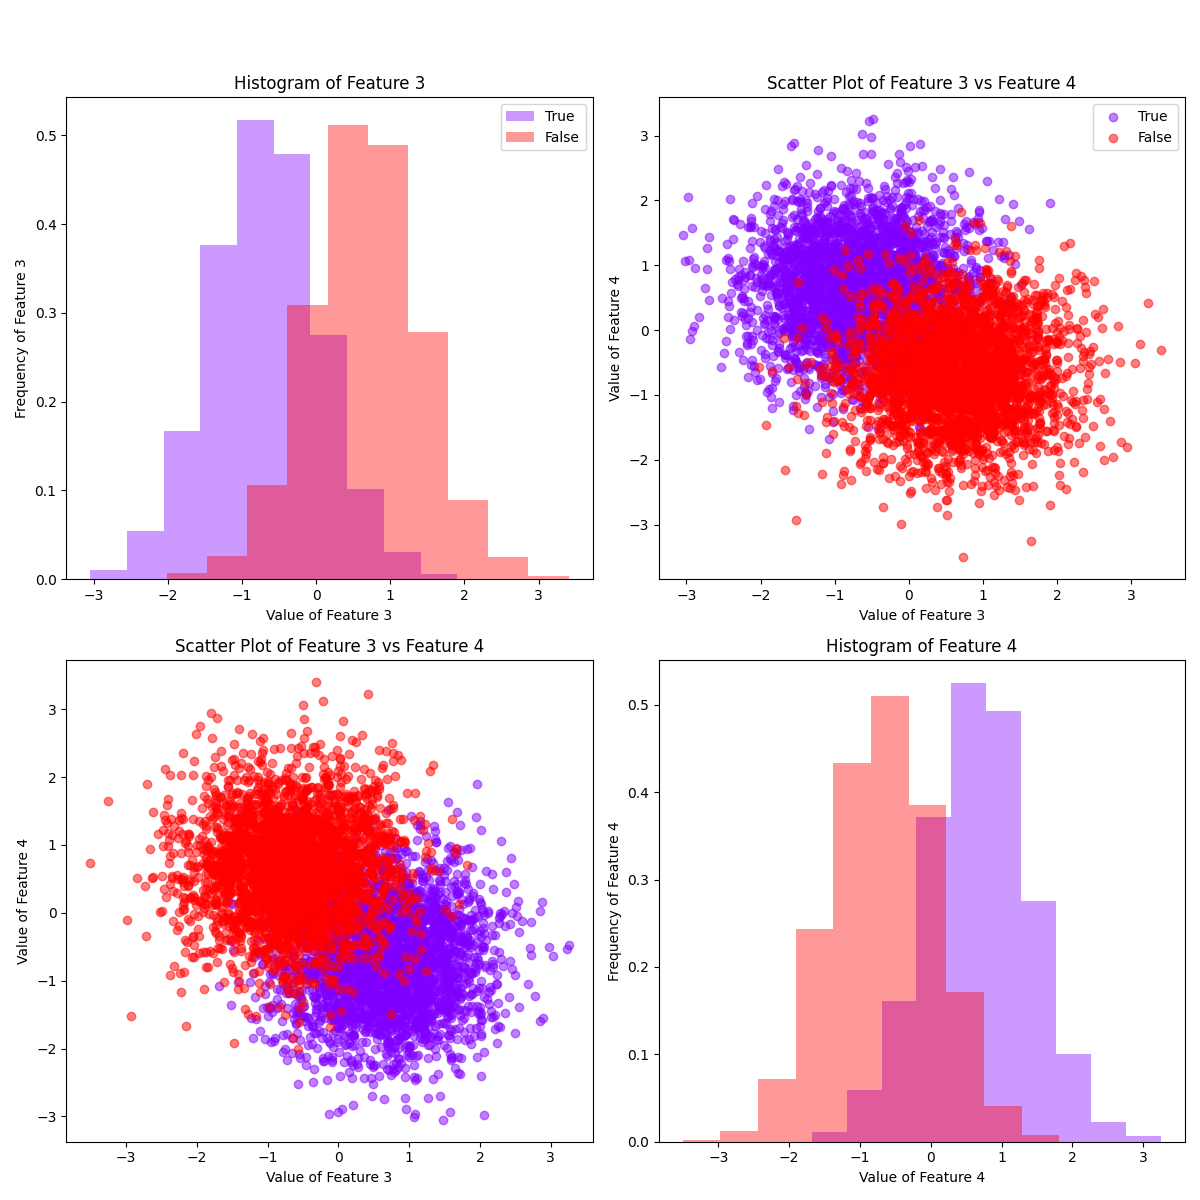
\includegraphics[width=0.7\linewidth]{img/projects/project1/3-4.png}
        \caption{Third and Fourth Features}
        \label{fig:project1_3-4}
    \end{figure}

    It is evident a less relevant overlap between the classes (although still present around the zero value) and four mode as before two for each feature and one for each class but, unlike the first two features, those modes are not overlapping, indicating a more robust distinction between the classes. Unlike the first two features, in both the third and fourth features the classes have similar variance (It is obvious that the mean is not equal as they don't completely overlap)
    Further mathematical analysis for the features are shown in the following table
    \begin{table}[htbp]
        \centering
        \begin{tabular}{|c|c|c|}
            \hline
            & \textbf{Feature 3}    & \textbf{Feature 4}    \\
            \hline
            \textbf{Mean}     & -0.005607526117533388 & 0.0010953708160571936 \\
            \hline
            \textbf{Variance} & 1.002481795216261     & 0.9902938938745539    \\
            \hline
        \end{tabular}
    \end{table}

    \subsubsection{Fifth and Sixth Features}
    \label{project1:3}

    Do the class overlap? If so, where? How many modes are evident from the histograms? How many clusters can you notice from the scatter plots for each class?

    Unlike already done in the previous answer, it is important to analyze both at the figure of the fifth and sixth features and then also at the table to better understand the details of those last two feature.

    \begin{figure}[h]
        \centering
        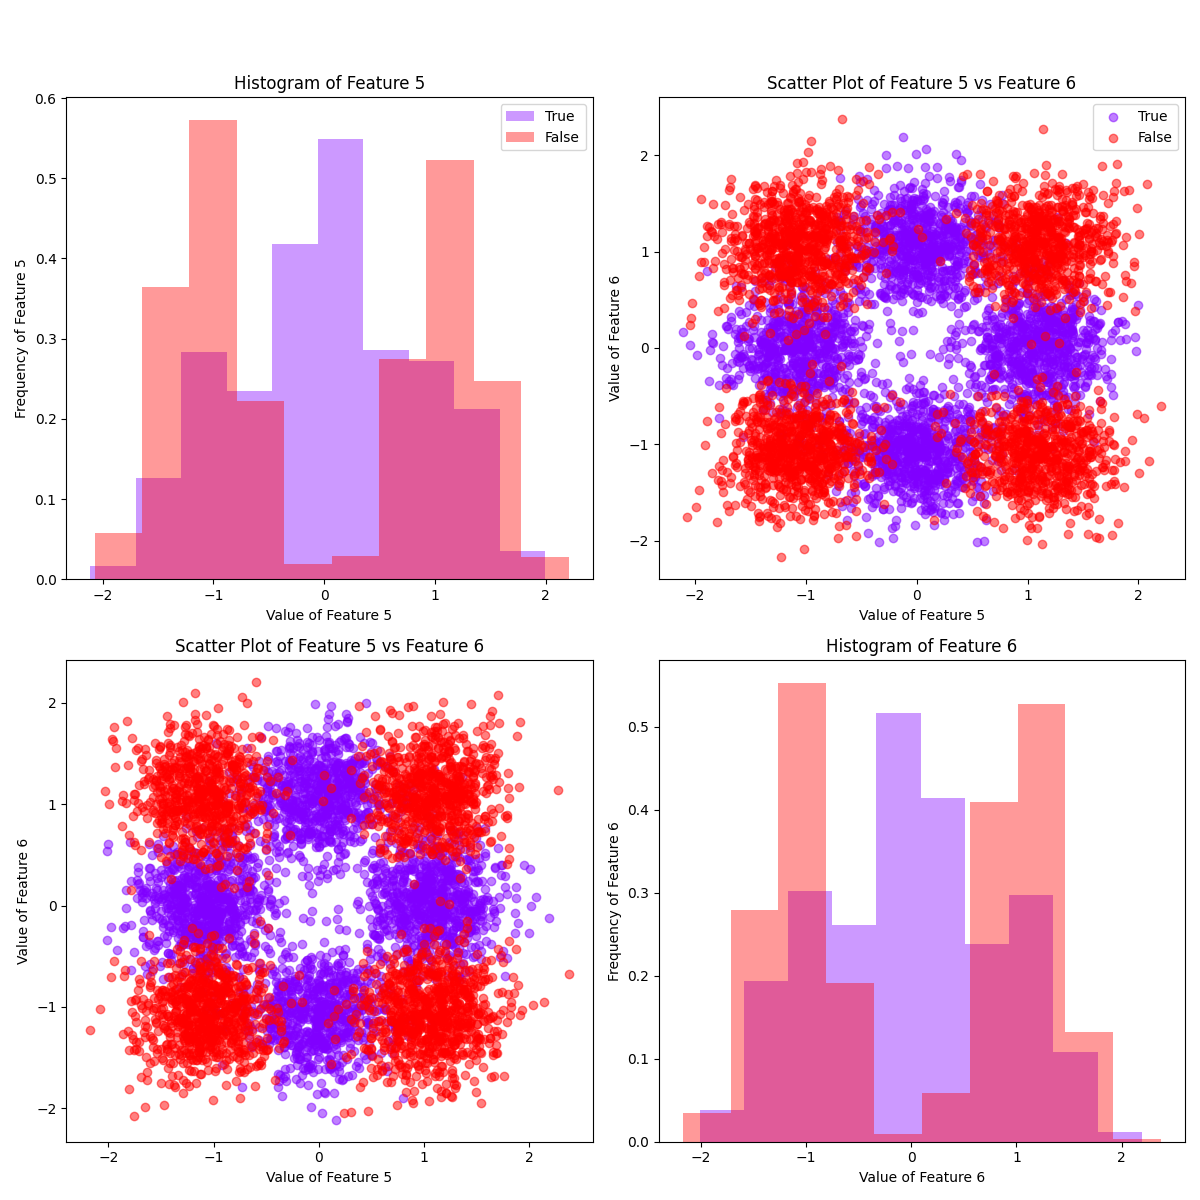
\includegraphics[width=0.7\linewidth]{img/projects/project1/5-6.png}
        \caption{Fifth and Sixth Features}
        \label{fig:project1_5-6}
    \end{figure}

    \begin{table}[htbp]
        \centering
        \begin{tabular}{|c|c|c|}
            \hline
            & \textbf{Feature 5}    & \textbf{Feature 6}   \\
            \hline
            \textbf{Mean}     & -0.007000246375933717 & 0.009105153611255263 \\
            \hline
            \textbf{Variance} & 1.0011974686052336    & 0.9972237418742479   \\
            \hline
        \end{tabular}
    \end{table}

    These metrics together indicate the importance of a visual approach when analyzing the features, as the mathematical approach alone would suggest (like it would have done for the previous features) a complete overlap of the features as their mean and variance are very similar.
    This is true as the mean is clearly around the zero value, but the actual distribution is much more interesting.
    The visual analysis reveals a possible of nine modes:
    \begin{enumerate}
        \item Four modes are very apparent and are evenly divided by the features, two for both of the \textbf{False} class.
        \item Two modes are also very apparent and are also evenly divided between the two feature, this time for the \textbf{True} class.
        \item The last three modes are much more subtle, all of them for the \textbf{True} class (one for the fifth feature and two for the sixth one) and overlap with the \textbf{False} class.
    \end{enumerate}

    The scatter plot reveals a clustering of the classes, dividing them in edges (\textbf{False} class) and borders (\textbf{True} class).


    \newpage


    \section{Project 2}

    \subsection{Questions}
    \begin{enumerate}
        \item Apply PCA and LDA to the project data. Start analyzing the effects of PCA on the features. Plot the histogram of the projected features for the 6 PCA directions, starting from the principal (largest variance). What do you observe? What are the effects on the class distributions? Can you spot the different clusters inside each class?
        \item Apply LDA (1 dimensional, since we have just two classes), and compute the histogram of the projected LDA samples. What do you observe? Do the classes overlap? Compared to the histograms of the 6 features you computed in Laboratory 2, is LDA finding a good direction with little class overlap?
        \item Try applying LDA as classifier. Divide the dataset in model training and validation sets (you can reuse the previous function to split the dataset). Apply LDA, select the orientation that results in the projected mean of class True (label 1) being larger than the projected mean of class False (label 0), and select the threshold as in the previous sections, i.e., as the average of the projected class means. Compute the predictions on the validation data, and the corresponding error rate.
        \item Now try changing the value of the threshold. What do you observe? Can you find values that improve the classification accuracy?
        \item Finally, try pre-processing the features with PCA. Apply PCA (estimated on the model training data only), and then classify the validation data with LDA. Analyze the performance as a function of the number of PCA dimensions m. What do you observe? Can you find values of m that improve the accuracy on the validation set? Is PCA beneficial for the task when combined with the LDA classifier?
    \end{enumerate}

    \subsection{Answers}

    \subsubsection{Answer 1}

    \newpage


    \section{Project 3}

    \subsection{Questions}
    \begin{enumerate}
        \item Try fitting uni-variate Gaussian models to the different features of the project dataset. For each component of the feature vectors, compute the ML estimate for the parameters of a 1D Gaussian distribution.
        \item Plot the distribution density (remember that you have to exponentiate the log-density) on top of the normalized histogram (set density=True when creating the histogram, see Laboratory 2). What do you observe? Are there features for which the Gaussian densities provide a good fit? Are there features for which the Gaussian model seems significantly less accurate?
    \end{enumerate}

    \subsection{Answers}

    \subsubsection{Answer 1}

    \newpage


    \section{Project 4}

    \subsection{Questions}
    \begin{enumerate}
        \item Apply the MVG model to the project data. Split the dataset in model training and validation subsets (\textbf{\textit{important}}: use the same splits for all models, including those presented in other laboratories), train the model parameters on the model training portion of the dataset and compute LLRs
        \[ s(\textbf{\textit{x}}_t) = llr(\textbf{\textit{x}}_t) =\dfrac{f_{\textbf{X}|C}(\textbf{x}_t|1)}{f_{\textbf{\textit{X}}|C}(\textbf{\textit{x}}_t|0)}\]
        (i.e., with class True, label 1 on top of the ratio) for the validation subset. Obtain predictions from LLRs assuming uniform class priors \(P(C = 1) = P(C = 0) = 1/2 \). Compute the corresponding error rate (suggestion: in the next laboratories we will modify the way we compute predictions from LLRs, we therefore recommend that you keep separated the functions that compute LLRs, those that compute predictions from LLRs and those that compute error rate from predictions).
        \item Apply now the tied Gaussian model, and compare the results with MVG and LDA. Which model seems to perform better?
        \item Finally, test the Naive Bayes Gaussian model. How does it compare with the previous two?
        \item Let’s now analyze the results in light of the characteristics of the features that we observed in previous laboratories. Start by printing the covariance matrix of each class (you can extract this from the MVG model parameters). The covariance matrices contain, on the diagonal, the variances for the different features, whereas the elements outside of the diagonal are the feature co-variances. For each class, compare the covariance of different feature pairs with the respective variances. What do you observe? Are co-variance values large or small compared to variances? To better visualize the strength of covariances with respect to variances we can compute, for a pair of features \(i, j\), the Pearson correlation coefficient, defined as
        \[ Corr(i,j) = \dfrac{Cov(i,j)}{\sqrt{Var(i)}\sqrt{Var(j)}}  \]
        or, directly matrix form,
        \textbf{Corr = C / ( vcol(C.diagonal()**0.5) * vrow(C.diagonal()**0.5) )}
        where \textbf{C} is a covariance matrix. The correlation matrix has diagonal elements equal to 1, whereas out-of-diagonal elements correspond to the correlation coefficients for all feature pairs, with \(1 \le Corr(i,j) \le 1\). When \(Corr(i,j) = 0\) the features \(i,j\) are uncorrelated, whereas values close to \(\pm1\) denote strong correlation.
        \item Compute the correlation matrices for the two classes. What can you conclude on the features? Are the features strongly or weakly correlated? How is this related to the Naive Bayes results?
        \item The Gaussian model assumes that features can be jointly modeled by Gaussian distributions. The goodness of the model is therefore strongly affected by the accuracy of this assumption. Although visualizing 6-dimensional distributions is unfeasible, we can analyze how well the assumption holds for single (or pairs) of features. In Laboratory 4 we separately fitted a Gaussian density over each feature for each class. This corresponds to the Naive Bayes model. What can you conclude on the goodness of the Gaussian assumption? Is it accurate for all the 6 features? Are there features for which the assumptions do not look good?
        \item To analyze if indeed the last set of features negatively affects our classifier because of poor modeling assumptions, we can try repeating the classification using only feature 1 to 4 (i.e., discarding the last 2 features). Repeat the analysis for the three models. What do you obtain? What can we conclude on discarding the last two features? Despite the inaccuracy of the assumption for these two features, are the Gaussian models still able to extract some useful information to improve classification accuracy?
        \item In Laboratory 2 and 4 we analyzed the distribution of features 1-2 and of features 3-4, finding that for features 1 and 2 means are similar but variances are not, whereas for features 3 and 4 the two classes mainly differ for the feature mean, but show similar variance. Furthermore, the features also show limited correlation for both classes. We can analyze how these characteristics of the features distribution affect the performance of the different approaches. Repeat the classification using only features 1-2 (jointly), and then do the same using only features 3-4 (jointly), and compare the results of the MVG and tied MVG models. In the first case, which model is better? And in the second case? How is this related to the characteristics of the two classifiers? Is the tied model effective at all for the first two features? Why? And the MVG? And for the second pair of features?
        \item Finally, we can analyze the effects of PCA as pre-processing. Use PCA to reduce the dimensionality of the feature space, and apply the three classification approaches. What do you observe? Is PCA effective for this dataset with the Gaussian models? Overall, what is the model that provided the best accuracy on the validation set?
    \end{enumerate}

    \subsection{Answers}

    \subsubsection{Answer 1}

    \newpage


    \section{Project 5}

    \subsection{Questions}
    \begin{enumerate}
        \item Start considering five applications, given by \((\pi_1,C_{fn},C_{fp})\):
        \begin{itemize}

            \item (0.5, 1.0, 1.0), i.e., uniform prior and costs
            \item (0.9, 1.0, 1.0), i.e., the prior probability of a genuine sample is higher (in our application, most users are legit)
            \item] (0.1, 1.0, 1.0), i.e., the prior probability of a fake sample is higher (in our application, most users are impostors)
            \item (0.5, 1.0, 9.0), i.e., the prior is uniform (same probability of a legit and fake sample), but the cost of accepting a fake image is larger (granting access to an impostor has a higher cost than labeling a legit user as an impostor - we aim for strong security)
            \item (0.5, 9.0, 1.0), i.e., the prior is uniform (same probability of a legit and fake sample), but the cost of rejecting a legit image is larger (granting access to an impostor has a lower cost than labeling a legit user as an impostor - we aim for ease of use for legit users)

        \end{itemize}
        Represent the applications in terms of effective prior. What do you obtain? Observe how the costs of mis-classifications are reflected in the prior: stronger security (higher false positive cost) corresponds to an equivalent lower prior probability of a legit user.
        \item We now focus on the three applications, represented in terms of effective priors (i.e., with costs of errors equal to 1) given by \(\widetilde{\pi} = 0.1\), \(\widetilde{\pi} = 0.5\) and \(\widetilde{\pi} = 0.9 \), respectively.
        \begin{enumerate}
            \item For each application, compute the optimal Bayes decisions for the validation set for the MVG models and its variants, with and without PCA (try different values of \textit{m}). Compute DCF (actual) and minimum DCF for the different models. Compare the models in terms of minimum DCF. Which models perform best? Are relative performance results consistent for the different applications? Now consider also actual DCFs. Are the models well calibrated (i.e., with a calibration loss in the range of few percents of the minimum DCF value) for the \textit{given applications}? Are there models that are better calibrated than others for the considered applications?
            \item Consider now the PCA setup that gave the best results for the \(\widetilde{\pi} = 0.1\) configuration (this will be our main application). Compute the Bayes error plots for the MVG, Tied and Naive Bayes Gaussian classifiers. Compare the minimum DCF of the three models for different applications, and, for each model, plot minimum and actual DCF. Consider prior log odds in the range \((-4,+4)\). What do you observe? Are model rankings consistent across applications (minimum DCF)? Are models well-calibrated over the considered range?
        \end{enumerate}


    \end{enumerate}

    \subsection{Answers}

    \subsubsection{Answer 1}

    \newpage


    \section{Project 6}

    \subsection{Questions}
    We analyze the binary logistic regression model on the project data. We start considering the standard, non-weighted version of the model, without any pre-processing.
    \begin{enumerate}
        \item Train the model using different values for \(\lambda\). You can build logarthimic-spaced values for \(\lambda\) using \textbf{numpy.logspace}. To obtain good coverage, you can use \textbf{numpy.logspace(-4, 2, 13)} (check the documentation). Train the model with each value of \(\lambda\), score the validation samples and compute the corresponding actual DCF and minimum DCF for the primary application \(\pi_T = 0.1\). \textit{To compute actual} DCF \textit{remember to remove the log-odds} of the training set empirical prior. Plot the two metrics as a function of \(\lambda\) (suggestion: use a logartihmic scale for the x-axis of the plot- to change the scale of the x-axis you can use \textbf{matplotlib.pyplot.xscale(’log’, base=10))}. What do you observe? Can you see significant differences for the different values of \(\lambda\)? How does the regularization coefficient affects the two metrics?
        \item Since we have a large number of samples, regularization seems ineffective, and actually degrades actual DCF since the regularized models tend to lose the probabilistic interpretation of the scores. To better understand the role of regularization, we analyze the results that we would obtain if we had fewer training samples. Repeat the previous analysis, but keep only 1 out of 50 model training samples, e.g. using data matrices \textbf{DTR[:, ::50], LTR[::50]} (apply the filter only on the model training samples, not on the validation samples, i.e., after splitting the dataset in model training and validation sets). What do you observe? Can you explain the results in this case? Remember that lower values of the regularizer imply larger risk of overfitting, while higher values of the regularizer reduce overfitting, but may lead to underfitting and to scores that lose their probabilistic interpretation.
        \item In the following we will again consider only the full dataset. Repeat the analysis with the prior-weighted version of the model (remember that, in this case, to transform the scores to LLRs you need to remove the log-odds of the prior that you chose when training the model). Are there significant differences for this task? Are there advantages using the prior-weighted model for our application (remember that the prior-weighted model requires that we know the target prior when we build the model)?
        \item Repeat the analysis with the quadratic logistic regression model (again, full dataset only). Expand the features, train and evaluate the models (you can focus on the standard, non prior-weighted model only, as the results you would obtain are similar for the two models), again considering different values for \(\lambda\). What do you observe? In this case is regularization effective? How does it affect the two metrics?
        \item The non-regularized model is invariant to affine transformations of the data. However, once we introduce a regularization term affine transformations of the data can lead to different results. Analyze the effects of centering (\underline{optionally}, you can also try different strategies, including Z-normalization and whitening, as well as PCA) on the model results. \textit{You can restrict the analysis to the linear model}. Remember that you have to center both datasets \textit{with respect to the model training dataset} mean, i.e., you must not use the validation data to estimate the pre-processing transformation. For this task, you should observe only minor variations, as the original features were already almost standardized.
        \item As you should have observed, the best models in terms of minimum DCF are not necessarily those that provide the best actual DCFs, i.e., they may present significant mis-calibration. We will deal with score calibration at the end of the course. For the moment, we focus on selecting the models that optimize the minimum DCF on our validation set. Compare all models that you have trained up to now, including Gaussian models, in terms of minDCF for the target application \(\pi_T = 0.1\). Which model(s) achieve(s) the best results? What kind of separation rules or distribution assumptions characterize this / these model(s)? How are the results related to the characteristics of the dataset features?
    \end{enumerate}

    \subsection{Answers}

    \subsubsection{Answer 1}

    \newpage


    \section{Project 7}

    \subsection{Questions}
    \begin{enumerate}
        \item Apply the SVM to the project data. Start with the linear model (to avoid excessive training time we consider only the models trained with \(K = 1.0\)). Train the model with different values of C. As for logistic regression, you should employ a logarithmic scale for the values of C. Reasonable values are given by \textbf{numpy.logspace(-5, 0, 11)}. Plot the minDCF and actDCF \((\pi_T = 0.1)\) as a function of C (again, use a logarithmic scale for the x-axis). What do you observe? Does the regularization coefficient significantly affect the results for one or both metrics (remember that, for SVM, low values of C imply strong regularization, while large values of C imply weak regularization)? Are the scores well calibrated for the target application? What can we conclude on linear SVM? How does it perform compared to other linear models? Repeat the analysis with centered data. Are the result significantly different?
        \item We now consider the polynomial kernel. For simplicity, we consider only the kernel with \(d = 2,c = 1\) (but better results may be possible with different configurations), and we set \(\xi = 0\), since the kernel already implicitly accounts for the bias term (due to \(c = 1\)). We also consider only the original, non-centered features (again, different pre-processing strategies may lead to better results). Train the model with different values of C, and compare the results in terms of minDCF and actDCF. What do you observe with quadratic models? In light of the characteristics of the dataset and of the classifier, are the results consistent with previous models (logistic regression and MVG models) in terms of minDCF? What about actDCF?
        \item For RBF kernel we need to optimize both \(\gamma\) and C (since the RBF kernel does not implicitly account for the bias term we set \(\xi = 1\)). We adopt a grid search approach, i.e., we consider different values of \(\gamma\) and different values of C, and try all possible combinations. For \(\gamma\) we suggest you analyze values \(\gamma \in [e^{-4},e^{-3},e^{-2},e^{-1}]\) , while for C, to avoid excessive time but obtain a good coverage of possible good values we suggest log-spaced values numpy.logspace(-3, 2, 11) (of course, you are free to experiment with other values if you so wish). Train all models obtained by combining the values of \(\gamma\) and of C. Plot minDCF and actDCF as a function of C, with a different line for each value of \(\gamma\) (i.e., four lines for minDCF and four lines for actDCF). Analyze the results. Are there values of \(\gamma\) and C that provide better results? Are the scores well calibrated? How the result compare to previous models? Are there characteristics of the dataset that can be better captured by RBF kernels?
    \end{enumerate}

    \subsection{Answers}

    \subsubsection{Answer 1}

    \newpage


    \section{Project 8}

    \subsection{Questions}
    \begin{enumerate}
        \item Question 1
    \end{enumerate}

    \subsection{Answers}

    \subsubsection{Answer 1}

    \newpage


    \section{Project 9}

    \subsection{Questions}
    \begin{enumerate}
        \item Question 1
    \end{enumerate}

    \subsection{Answers}

    \subsubsection{Answer 1}

%********************************%
%***********References***********%
%********************************%
    \newpage
% \patchcmd{\thebibliography}{\section*}{\section}{}{}
% Now we need a bibliography:
    \printbibliography

    \noindent
\end{document}